\chapter{Open Air Museum} % senza numerazione
\label{Open Air Museum}

\vspace{5mm}

\section{App nativa}\vspace{5mm}

L’applicazione consiste in una guida turistica e multimediale in grado di mostrare ai suoi utenti una serie di punti di interesse collegati da percorsi preimpostati. Ogni punto dispone di un pacchetto multimediale di audio e immagini oltre ad una descrizione, un nome e delle informazioni tutte gestibili e configurabili in oltre 160 lingue. Tali punti possono essere navigati attraverso l’interfaccia grafica degli applicativi per smartphone - sfruttando la geolocalizzazione del dispositivo - oppure attraverso la modalità Esplora dell’applicazione. Quest'ultima permette, una volta attivata, di essere notificati automaticamente sulla presenza di punti di interesse nella zona circostante, dando la possibilità, o meno, all’utente di richiedere informazioni aggiuntive. Questo è possibile grazie a due componenti, la tecnologia iBeacon, che descriverò in seguito, e il background processing. Quest'ultimo è stato implementato mediante la registrazione di una background task per la localizzazione, tale procedura permette all'applicativo di registrare all'interno del sistema operativo una finestra di esecuzione dedita a quell'operazione specifica. Tale implementazione permette di risparmiare batteria essendo controllabile quasi interamente dal sistema operativo. Infatti se il sistema necessita di nuove risorse o in altri casi limite potrebbe interrompere la task in background.\vspace{5mm}

\section{iBeacon}\vspace{5mm}

La modalità esplora citata nella sezione sopra è stata implementata sfruttando la tecnologia iBeacon e Bluetooth 4.0, che permette al dispositivo di percepire l’ingresso in una specifica area, marcata da un piccolo radiofaro bluetooth, il quale marca di fatto un determinato punto di interesse.\vspace{5mm}

La metodologia con cui viene identificata una zona rispetto ad un altra è usando la firma del Beacon e cioè attraverso i suoi tre parametri identificativi, UUID, major e minor. Il primo è una stringa alfanumerica a 128 bit che ha lo scopo di identificare un gruppo di Beacon, ad esempio l’insieme posizionato all’interno del comune, mentre gli ultimi due, insieme all’UUID identificano un beacon specifico. Utilizzando lo UUID per definire una Ragion di ricerca è possibile escludere da essa tutti gli altri beacon non appartenenti all’applicativo. Infatti tutti i beacon da noi posizionati sono contraddistinti da uno specifico UUID mentre differiscono per major e minor, in modo da identificarli singolarmente. Un ulteriore metodo per gestire la “scoperta” di beacon in una regione è quello di verificarne la distanza dal telefono, così facendo si possono scartare i beacon più lontani e notificare all’utente solamente quelli più prossimi, questo è fondamentale dato che vi sono delle zone della città molto “dense” di punti di interesse e una semplice ricerca non basterebbe a definire la prossimità di un utente a un punto rispetto ad un altro; questa features ha aiutato a realizzare una localizzazione più precisa e risultando in un’esperienza d’uso migliore.\vspace{5mm}

\section{Software gestionale}\vspace{5mm}

	Attraverso l’applicativo in Filemaker, esposto tramite un’interfaccia web, i dipendenti del Comune potevano gestire l’inserimento dei punti e dei percorsi compresi di media e testi relativi. \vspace{5mm}
	
La visualizzazione dei punti avviene attraverso due schermate, la prima è una lista che mostra tutti i punti con un ordine casuale e vi è la possibilità di navigare ad una schermata più dettagliata dove vi sono le informazioni del punto selezionato ed è possibile riprodurre i contenuti multimediali associati ad esso. La seconda mostra l'elenco di tutti i percorsi disponibili, dando la possibilità, una volta selezionato, di vedere nel dettaglio di quali punti è composto e in che ordine visitarli. Per ogni testo vi è la possibilità di indicare una traduzione in tutte le lingue supportate dall'applicativo, tedesco, inglese, spagnolo, cinese semplificato, russo e italiano. Tali traduzioni non sono svolte in maniera automatica ma devono essere inserite manualmente; questo per dare maggiore controllo al dipendente comunale che inserisce i dati.\vspace{5mm}

Filemaker mette a disposizione un interfaccia drag and drop per la creazione della parte visuale dell'applicativo, permettendo di collegare i vari elementi trascinati nell'area di lavoro ad una specifica entry di un database. Tale interfaccia viene quindi tenuta sempre in sincronia dal motore di Filemaker per riflettere i dati contenuti nel database; questo permette di avere un interfaccia facilmente modificabile e una raccolta dati consistente.\vspace{5mm}

Un ulteriore features di questo prodotto è la possibilità di convertirlo in una web application; questo permette a chiunque possegga un dispositivo in grado di avere un browser in grado di sfruttare questa piattaforma per il caricamento dei dati. Tale scelta si è rivolta vincente vista la grande frammentazione dei dispositivi in uso negli uffici della suddetta P.A.; non vi sono infatti requisiti particolari per l'utilizzo di tale piattaforma.

\section{Server}\vspace{5mm}
	
La parte server, invece, espone delle Rest Api che consumate forniscono sia i dati sopracitati che un servizio di autenticazione mediante Json Web Token. Questo applicativo è stato sviluppato senza l’ausilio di framework esterni per il routing o per la gestione dell’autenticazione o la generazione dei token di sessione. Node Js è stato scelto in questo caso per la sua efficienza nelle operazioni di I/O rispetto ad una tecnologia più canonica come PHP o Java, vista la grande quantità e la tipologia di file da servire. Implementando un I/O non bloccante\cite{BlockingVsNonBlocking} nel caso di invio di file di medie dimensioni come audio o immagini questo risulta nel riuscire a servire più client contemporaneamente utilizzando meno risorse. Tale applicativo utilizza il file system della macchina per salvare tutti i media che comprendono immagini e audio. Tali media sono serviti utilizzando il file system come base e mediante l'interfaccia messa a disposizione da Nodejs vengono serviti attraverso una specifica Api http. I media sono salvati all'interno di un database MySql attraverso il percorso che hanno nel file system rispetto alla radice del progetto. Questo approccio permette di svicolare il database da una task onerosa come quella di dover convertire i file ricevuti in base64 e salvandoli come entry tabellare. Tale procedura inserisce una criticità, cioè che i dati presenti nella memoria possono non riflettere quelli salvati a database e vice versa, perchè non vi è una correlazione diretta tra i due dati. Le api sono state disegnate per simulare questa correlazione, questo coadiuvato da un blocco di operazioni di lettura e scrittura nella specifica directory mantengono i media e i dati a database in sincronia. Il blocco sulla lettura e scrittura è fatto attraverso le impostazioni di lettura e scrittura di linux delegando al solo utente che ospita il processo Nodejs, che è il server, a poter leggere e scrivere in tale cartella.\vspace{5mm}

L'autenticazione come detto in precedenza avviene attraverso una tecnica chiamata Json Web Token\cite{JWT}. Consiste in uno standard open source basato su JSON per la creazione di token di accesso, questi token sono firmati per essere piccoli e criptati mediante una chiave privata cosi da essere decodificati solamente dalle parti autorizzate. Sono generati per essere URL-safe e per eseguire piccole transazioni di dati o per provare un autorizzazione. Nel caso di Open Air Museum vengono utilizzati per validare l'autenticazione. Fin quando un token resta valido e cioè che la sua data di scadenza non è passata il client che lo conserva può utilizzarlo per autenticare tutte le richieste. Per fare questo ogni richiesta http dovrà contenere nell'header di essa la chiave 'Authorization' con valore 'Bearer' seguito da uno spazio e il token. Tale autenticazione di fatto implementa lo standard RFC 6750: OAuth 2.0 Bearer Token\cite{Bearer}.

\begin{figure}[h]
\centering
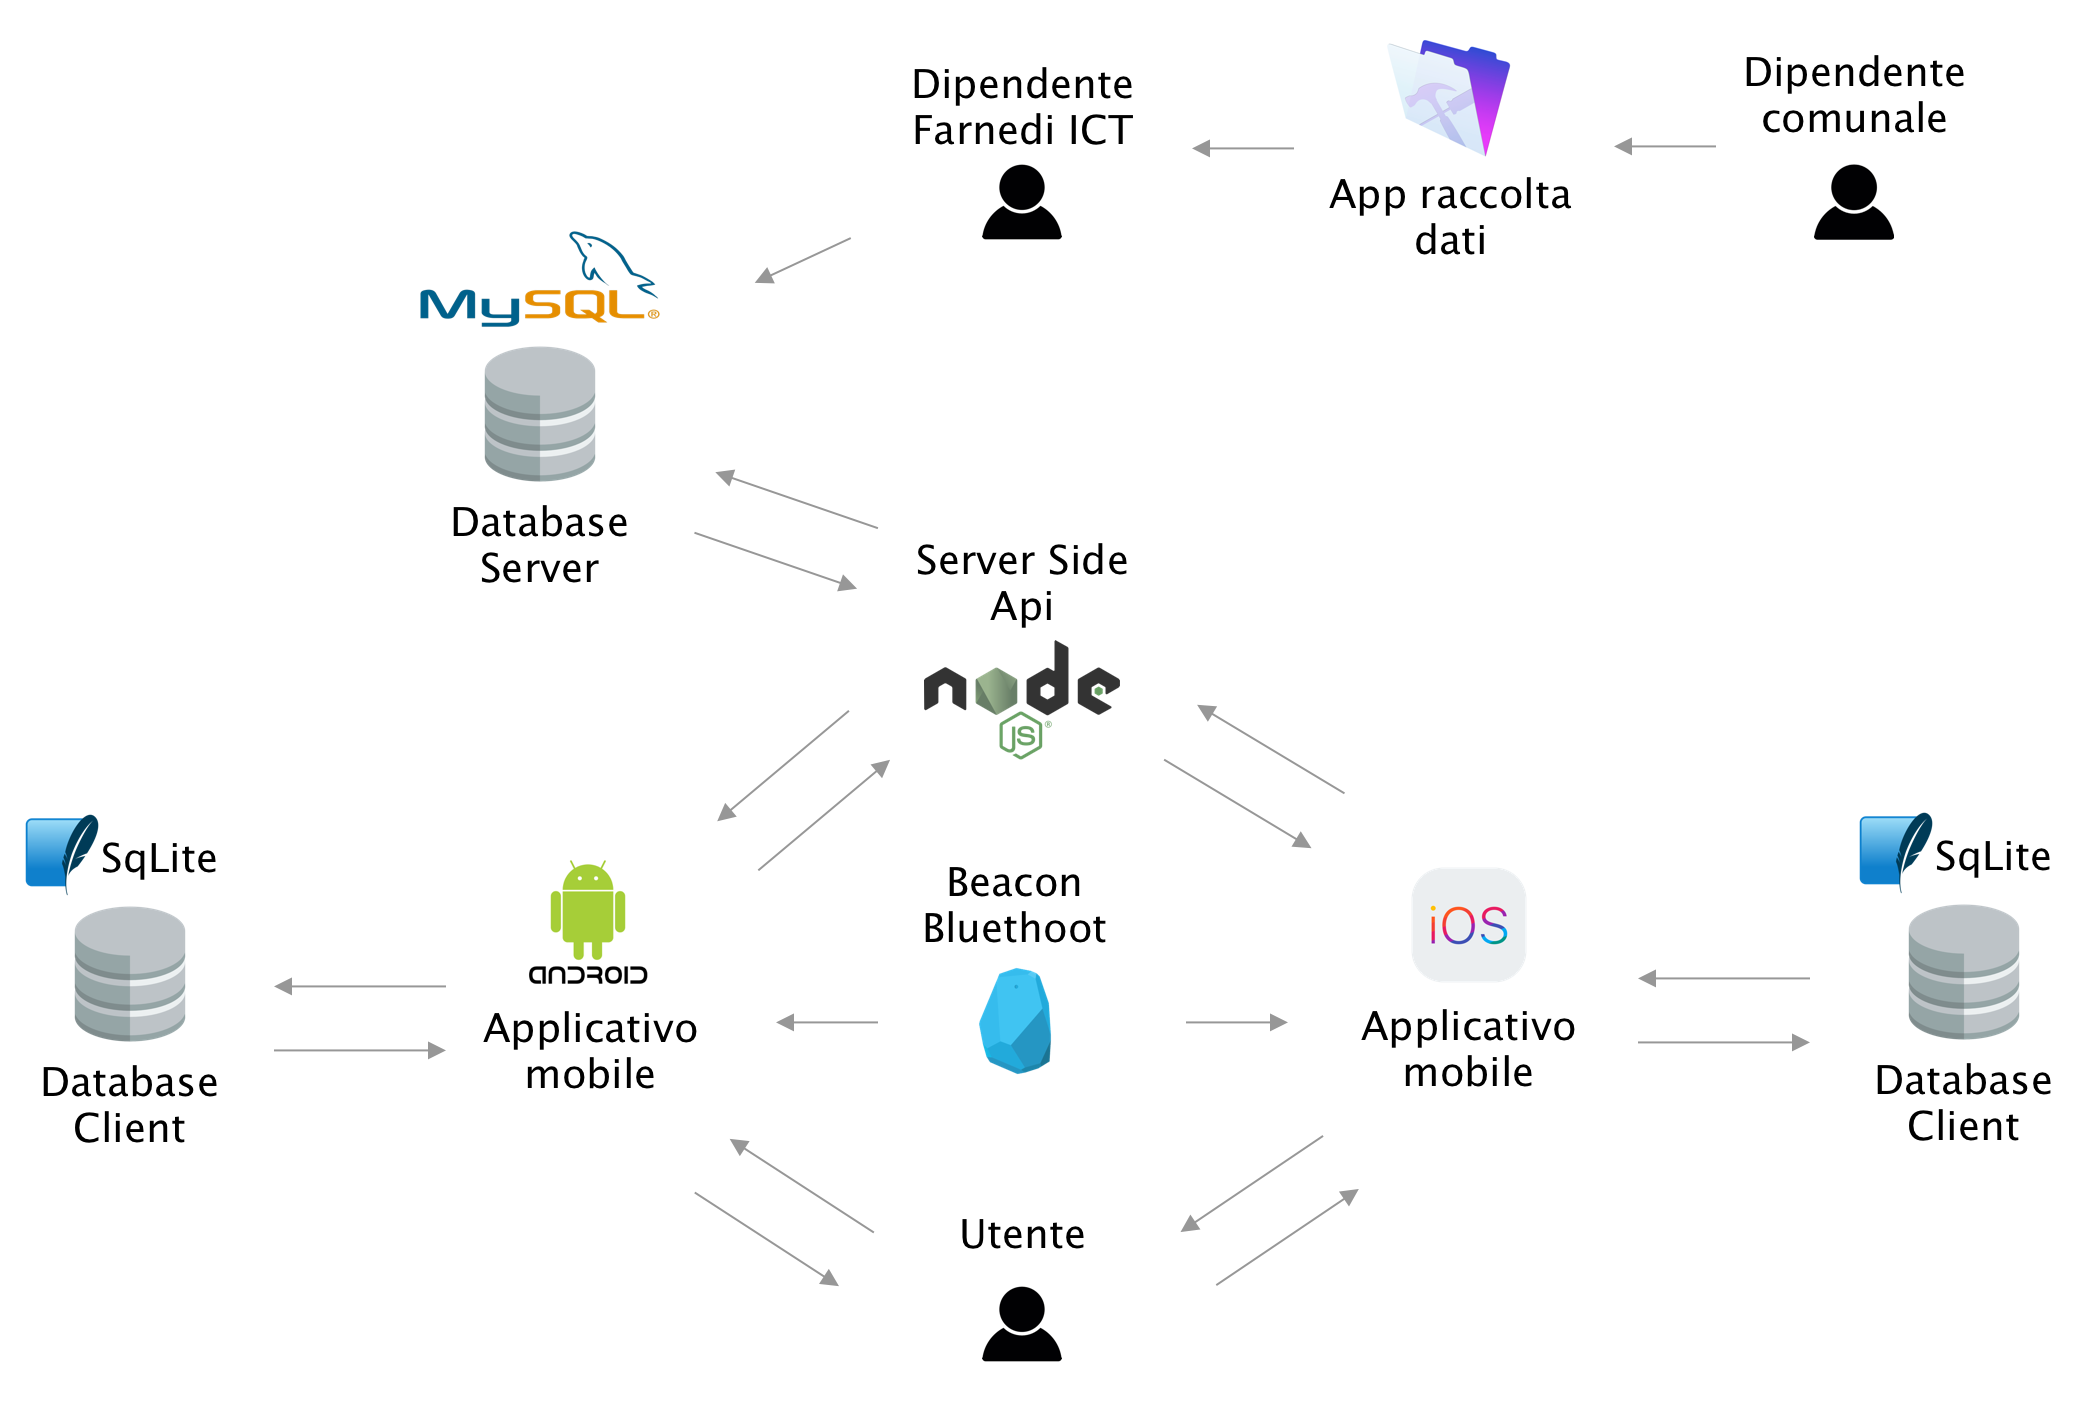
\includegraphics[width=0.9\textwidth]{images/SchemaOpenAirMuseum.png}
\caption{Schema logico dello stack di Open Air Museum}
\end{figure}







